\chapter{Transactions}

\begin{definition}
   [Transaction]
   A \textbf{transaction} is a sequence of operations that are executed as a single unit of work. A transaction can consist of multiple operations, such as reads, writes, and updates.
   A transaction has to be \textbf{atomic}: all the operations in the transaction are executed successfully or none of them are.\\
   Besides, when a transaction is executed on some data, none of the other transactions can alter that data until the transaction is completed.
\end{definition}

Transactions are clearly crucial in a distributed system, as they build a framework for allowing to maintain data consistency across multiple nodes.



% Lesson 14/11
Transactions come at a cost, since in a distributed system even a simple mechanism such as a mutex may become costly to implement.\\
Transactions hence provide all-or-nothing guarantees, simplifying \textbf{error handling}, since partial failures are not to be managed.




\section{Deeper into DBs}

Most SQL DBs support transactions.
NoSQL databases typically do not support transactions, but some of them provide limited support for transactions on a single object.
\subsection{Why NoSQL DBs do not support transactions?}
NoSQL databases typically do not support transactions because they are designed to be highly scalable and distributed,
and transactions can be difficult to implement in a distributed system.
Transactions require coordination between multiple nodes, which can be costly and can lead to performance issues.

NoSQL databases typically prioritize scalability and performance over strong consistency guarantees, which are provided by transactions.
However, some NoSQL databases provide limited support for transactions on a single object, which can be useful for certain applications.



\section{ACID Properties}

\begin{itemize}
    \item \textbf{Atomicity}: all operations in a transaction are executed successfully or none of them are.
    \item \textbf{Consistency}: the database is in a consistent state before and after the transaction.
    \item \textbf{Isolation}: the transaction is executed in isolation from other transactions.
    \note{In other words, transactions appear to run serially}
    \item \textbf{Durability}: once a transaction is committed, the changes are permanent.
    \note{Perfect durability is unattainable}
\end{itemize}

These were coined by \textit{Jim Gray} in 1983.

\subsection{Durability}
Durability is the property that ensures that once a transaction is committed, the changes are permanent.

This is a mess to ensure and in general is not possible to guarantee, but it is possible to make it very unlikely that a transaction is lost.

The issue is related to hardware faults, power outages, broken firmware,\dots\\
Given the absence of a one-size-fits-all solution, typically the approach involves a combination of writing to disk, replicating to remote machines, and backups.

\subsection{Single-Object and Multi-Object Transactions}
If a \ul{transaction involves multiple objects, it is a multi-object transaction, which causes \textbf{performance} and \textbf{deadlock} issues.}


Databases hide concurrency issues by providing transaction isolation.
Isolation allows the application to pretend that no concurrency is happening.
\ul{Serializable isolation guarantees that the transactions are executed in a serial order, which is the most strict isolation level.}

Serializable isolation comes with a performance cost which makes it less common in practice.
Weaker isolation levels are common, but are harder to understand and may lead to subtle bugs.

\section{Avoiding Transactions}
\subsection{Read Committed}
In \textit{Read Committed} isolation level, a transaction can only read, and overwrite, committed data.
This is the default isolation level in most databases.

\begin{definition}
   [Dirty Read]
   A \textbf{dirty read} occurs when a transaction reads data that has been written by another transaction that has not yet been committed.
\end{definition}


\begin{definition}
   [Dirty Write]
   A \textbf{dirty write} occurs when a transaction overwrites data that has been written by another transaction that has not yet been committed.
\end{definition}

In this model, \ul{\textbf{no} dirty reads nor dirty writes are allowed}.

% This model is not enough to prevent \textbf{non-repeatable reads} and \textbf{phantom reads}.
This model is more reliable than Non-transactional models, but still allows to avoid ``paying'' for transactions.

\begin{definition}
   [Non-repeatable Read]
   A \textbf{non-repeatable read} occurs when a transaction reads the same data twice and gets different results.
\end{definition}

Non-repeatable reads are possible in \textit{Read Committed} isolation level, 

\begin{figure}[htbp]
   \centering
   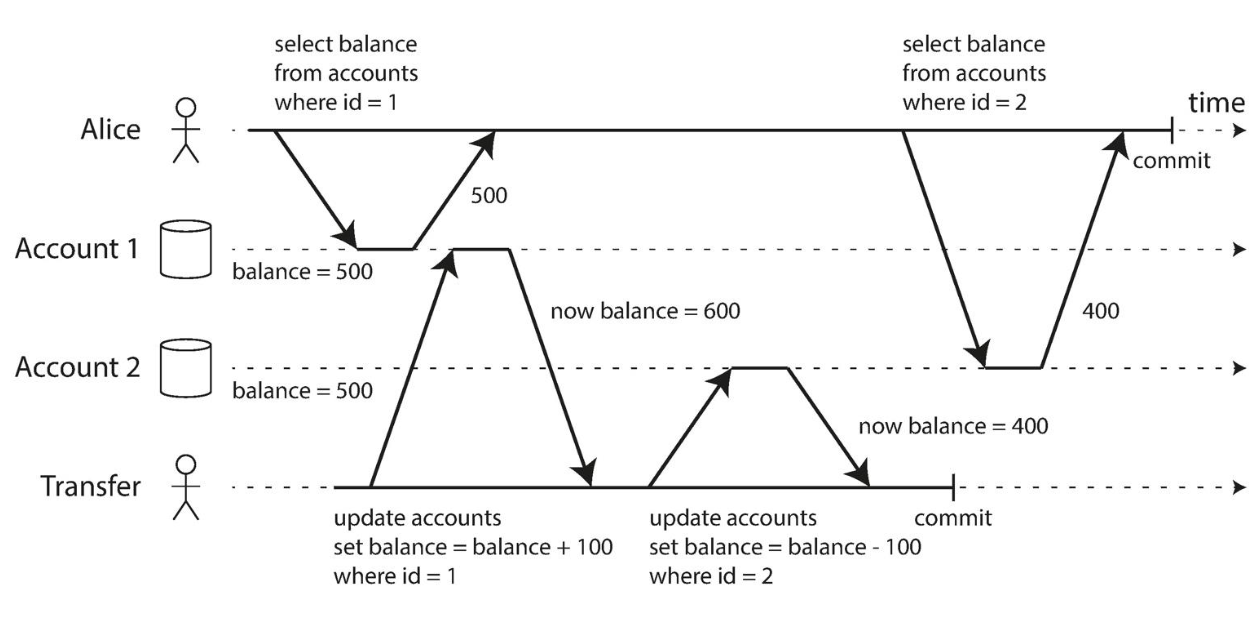
\includegraphics{images/12/readcommitted_issue.png}
   \caption{Read committed issue: Alice might think that her whole balance is 900, whilst it is 1000.}
   \label{fig:12/readcommitted_issue}
\end{figure}
% \begin{definition}
%    [Phantom Read]
%    A \textbf{phantom read} occurs when a transaction reads a set of records that satisfy a certain condition, but when it reads the same records again, the set of records has changed.

\subsection{Snapshot Isolation}
\textit{Snapshot Isolation} is a more relaxed isolation level than serializable isolation, but it is still stricter than \textit{Read Committed} isolation.

In \textit{Snapshot Isolation}, a transaction reads a snapshot of the database at the beginning of the transaction and writes to the database at the end of the transaction.

The snapshot allows transactions to see all the data that was commited at the start of the transaction.

% // TODO there is some other stuff about explicit locks, I'm not sure how important it is, the slides are a bit messed up

\note{It is possible to use some techniques for locking the database, using locks or atomic operations. 
However it is costful}

This model implements isolation by means of a lock to prevent dirty writes, but allows dirty reads (?), since reads do not acquire any locks.
Readers never block writers, and writers never block readers.\\
Along with locks, MVCC (Multi-Version Concurrency Control) is used to provide each transaction with a snapshot of the database at the start of the transaction.
In practice, each write creates a new version of the object, and the old version is kept around for readers that started before the write.

Compared to \textit{Read Committed}, we could say that while \textit{Read Committed} uses a \ul{separate snapshot for each \textbf{query}}, \textit{Snapshot Isolation} uses a \ul{single snapshot for the whole \textbf{transaction}}.

\section{Write Skew and Phantoms}

\begin{paracol}{2}
  
   \colfill
   \begin{definition}
      [Write Skew]
      A \textbf{write skew} occurs when two transactions read the same data, then update ---possibly separate--- objects based on the read data, and then commit, causing a conflict.
   \end{definition}
   There are some techniques to avoid write skew, such as using row locks, atomic operations, or specific constraints, but we did not discuss them pretty much.
   \colfill
   
   \switchcolumn

   \begin{figure}[htbp]
      \centering
      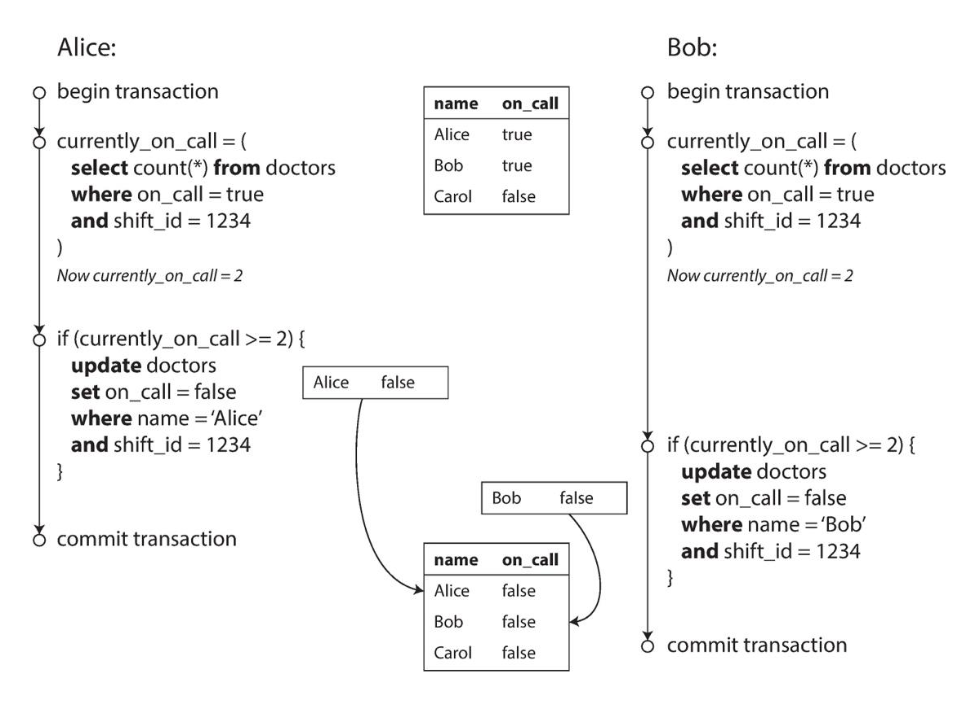
\includegraphics[width=0.9\columnwidth]{images/12/write_skew.png}
      \caption{Both doctors read that \lstinline|currently_on_call >= 2| and ``leave the hospital'', causing no doctor to be on call \frownie.}
      \label{fig:12/write_skew}
   \end{figure}
\end{paracol}



